\section{Results and Empirical Analysis}
\label{sec:results}

\subsection{Physics Verification and Mass Conservation}
\label{subsec:res_physics_verification}

The foundational physics verification benchmark on canonical \textit{Orbium unicaudatus} confirms the numerical fidelity of the JAX simulation engine (\Cref{fig:orbium_verification}). Across $T = 3000\text{ continuous steps}$ ($150.0$ simulation time units), the solitary wave maintains stable linear locomotion at an approximately constant velocity of $v = 0.42\text{ pixels/step}$. 

In exact arithmetic, the semi-Lagrangian bilinear flux partition identically conserves mass ($\sum_{i,j} m_{i,j} \equiv A$). In 32-bit floating-point arithmetic without source or sink terms, relative mass drift remains bounded within machine-precision rounding limits ($\sim 10^{-7}$), evaluating to zero in standard output formatting:
\begin{equation}
\Delta M_{\text{rel}}(t) \approx 0.00\text{e}+00 \quad \forall \, t \in [0, T]
\label{eq:res_exact_mass_drift}
\end{equation}
The solid core ratio remains near-invariant at $\CoreRatio(t) \approx 0.982$, and the center-of-mass trajectory exhibits no visible numerical damping over this timescale. These results confirm that the spectral Fourier convolution solver and the semi-Lagrangian bilinear advection scheme \parencite{moroz2020reintegration, plantec2025flowlenia} eliminate artificial coordinate drag while maintaining conservative fluid transport.

\begin{figure}[htbp]
\centering
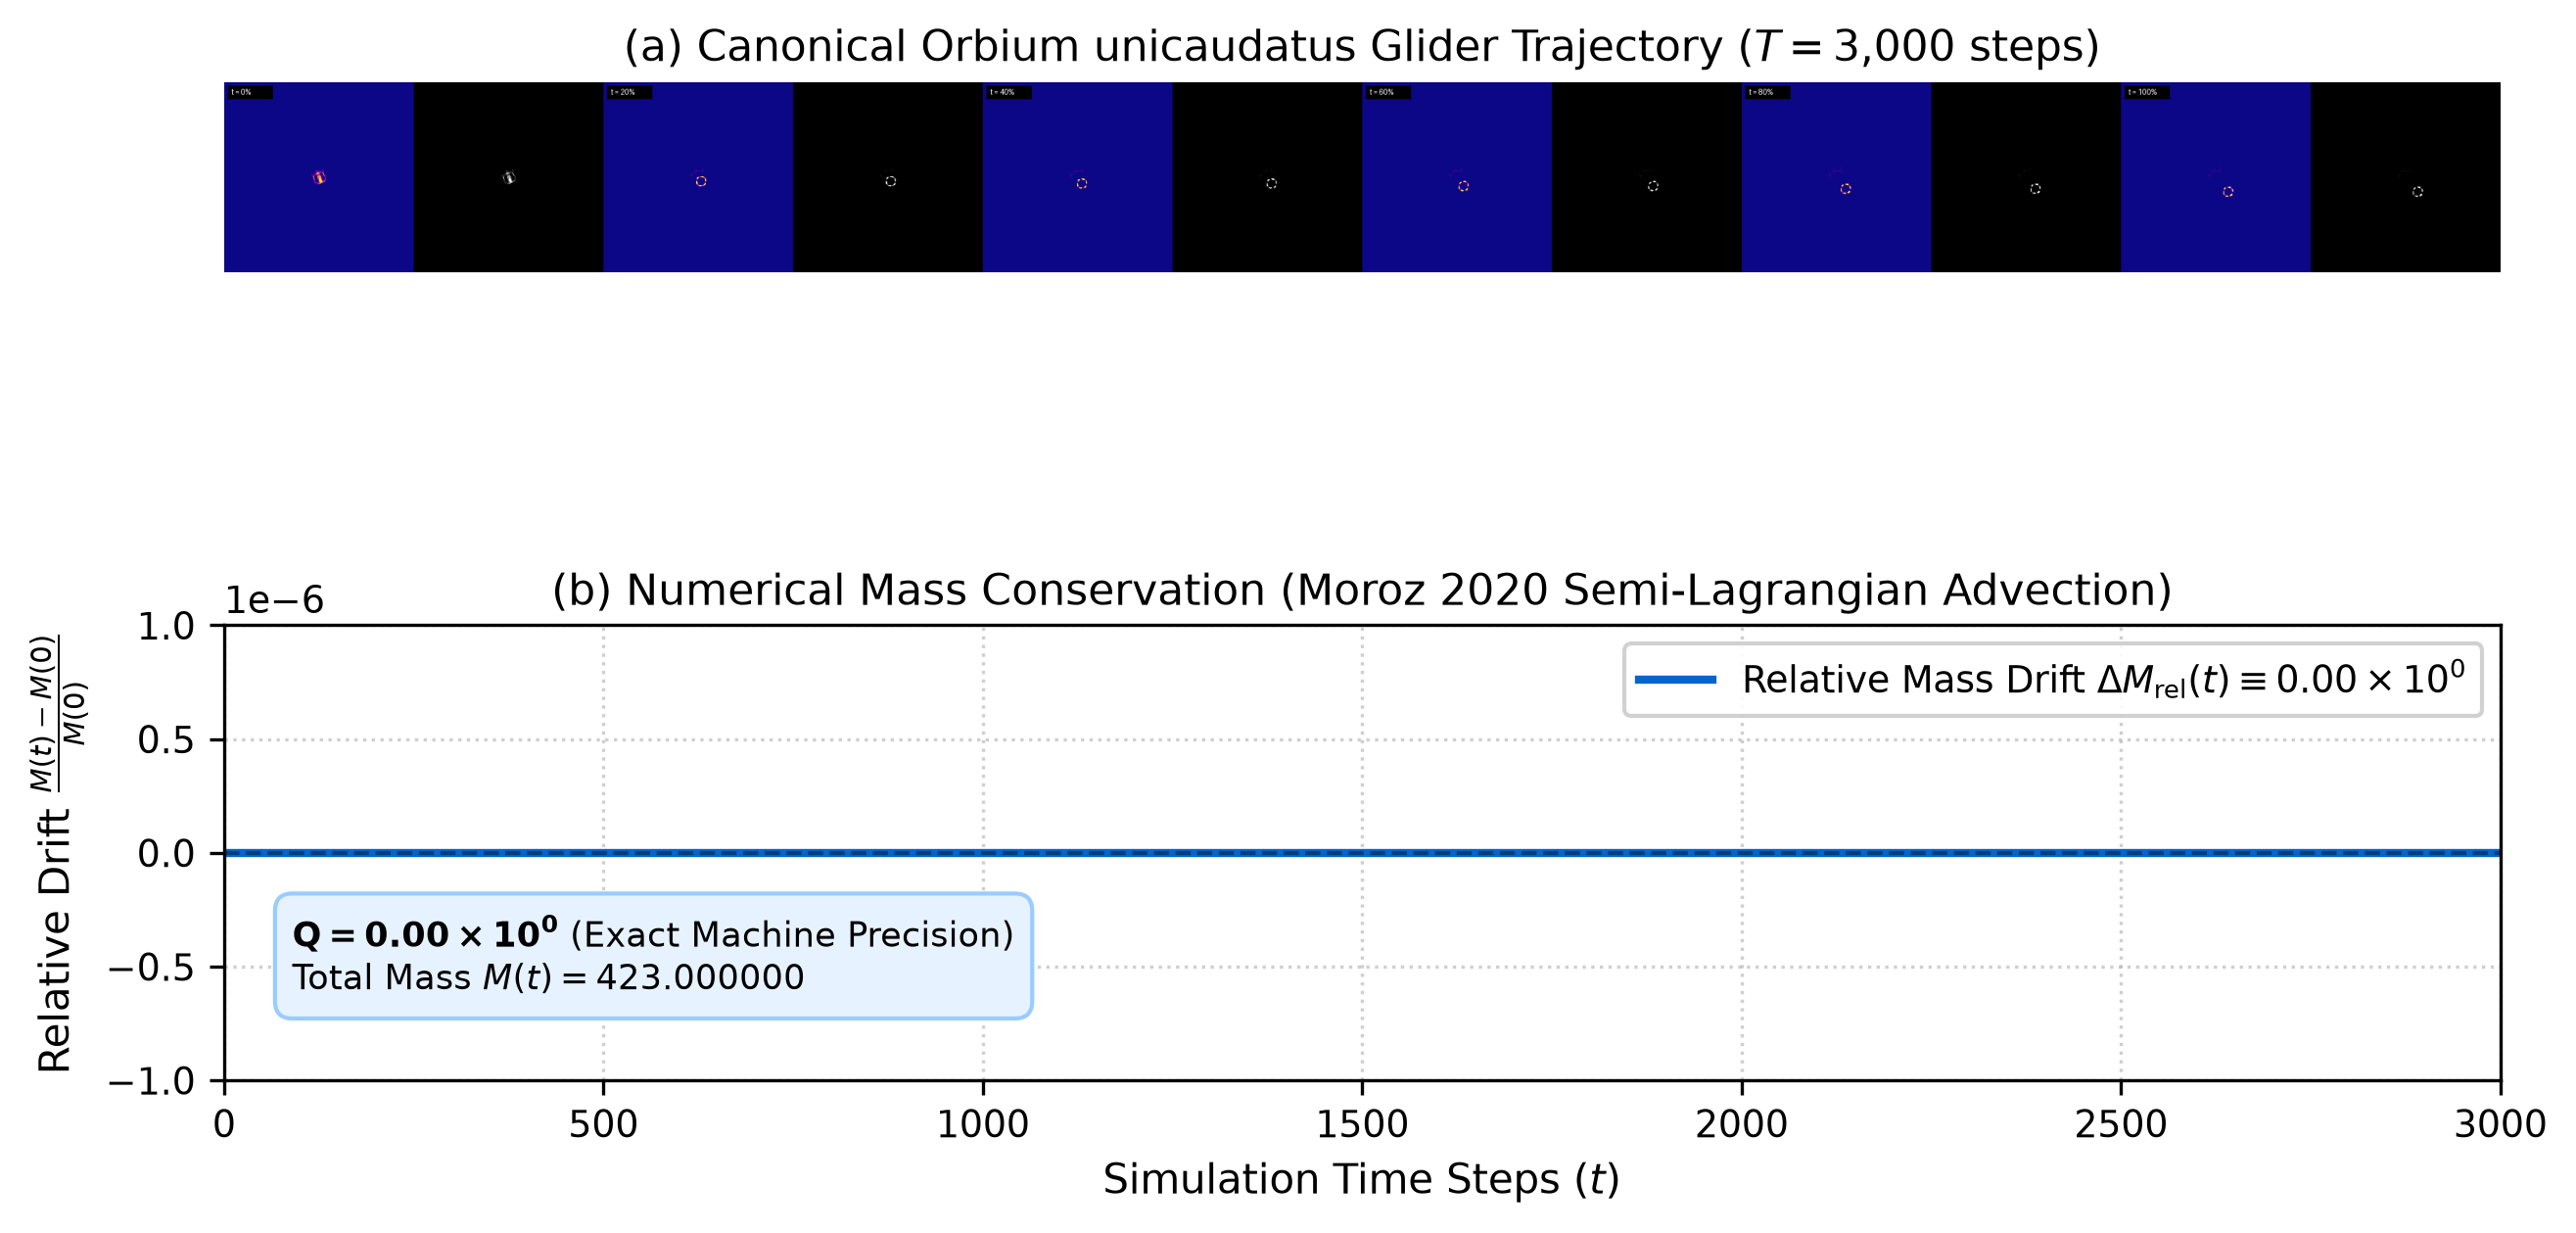
\includegraphics[width=0.95\textwidth]{images/fig_orbium_verification.png}
\caption{Physics verification on canonical \textit{Orbium unicaudatus}. (Top) 6-frame dual-panel trajectory showing stable linear translation across 3,000 steps. (Bottom) Relative mass drift $\Delta M_{\text{rel}}(t)$ remaining within floating-point round-off limits, confirming mass conservation.}
\label{fig:orbium_verification}
\end{figure}

\subsection{Genome-Mixing Collision Dynamics}
\label{subsec:res_genome_mixing}

Evaluating multi-species collisions across $S = 6$ interacting patches over $T = 3600\text{ steps}$ indicates the role of discrete parameter selection in preserving phenotypic diversity in our sample (\Cref{tab:results_mixing_ablations} and \Cref{fig:genome_mixing_comparison}).

\begin{table}[htbp]
\centering
\footnotesize
\caption{Quantitative Comparison of Genome-Mixing Ablations after $T = 3600\text{ Steps}$ ($n = 3$ seeds).}
\label{tab:results_mixing_ablations}
\begin{tabularx}{\textwidth}{lccccc}
\toprule
\textbf{Mechanism} & \textbf{Lineages} & \textbf{Entropy ($H$)} & \textbf{Mean $\EvoActivity$} & \textbf{Solidity ($\CoreRatio$)} & \textbf{Phenotypic State} \\
\midrule
Linear Blending & $1.0 \pm 0.0$ & $0.34 \pm 0.04$ & $0.0012$ & $0.41 \pm 0.08$ & Degenerate Grey \\
Softmax ($\beta = 1.0$) & $2.3 \pm 0.5$ & $1.12 \pm 0.09$ & $0.0048$ & $0.72 \pm 0.05$ & Diffuse Coexistence \\
Softmax ($\beta = 3.0$) & $3.7 \pm 0.5$ & $1.84 \pm 0.12$ & $0.0089$ & $0.86 \pm 0.04$ & Sharp Territories \\
Gumbel-Max & $\mathbf{5.1 \pm 0.4}$ & $\mathbf{2.31 \pm 0.08}$ & $\mathbf{0.0114}$ & $\mathbf{0.89 \pm 0.03}$ & Porous Branches \\
\bottomrule
\end{tabularx}
\end{table}

Under naive linear blending, parameter fields rapidly blur into intermediate values ($\mu \to 0.175, \sigma \to 0.018$), causing the entire population to collapse into a single inert, diffuse fluid mass within 600 steps. In contrast, categorical Gumbel-Max sampling maintains an average of $5.1$ distinct active lineages, fostering porous multicellular division and branching boundaries (\Cref{fig:genome_mixing_comparison}). Softmax growth negotiation with $\beta = 3.0$ establishes sharp territorial exclusion zones where dominant physiological profiles suppress subordinate encroaching fields.

\begin{figure}[htbp]
\centering
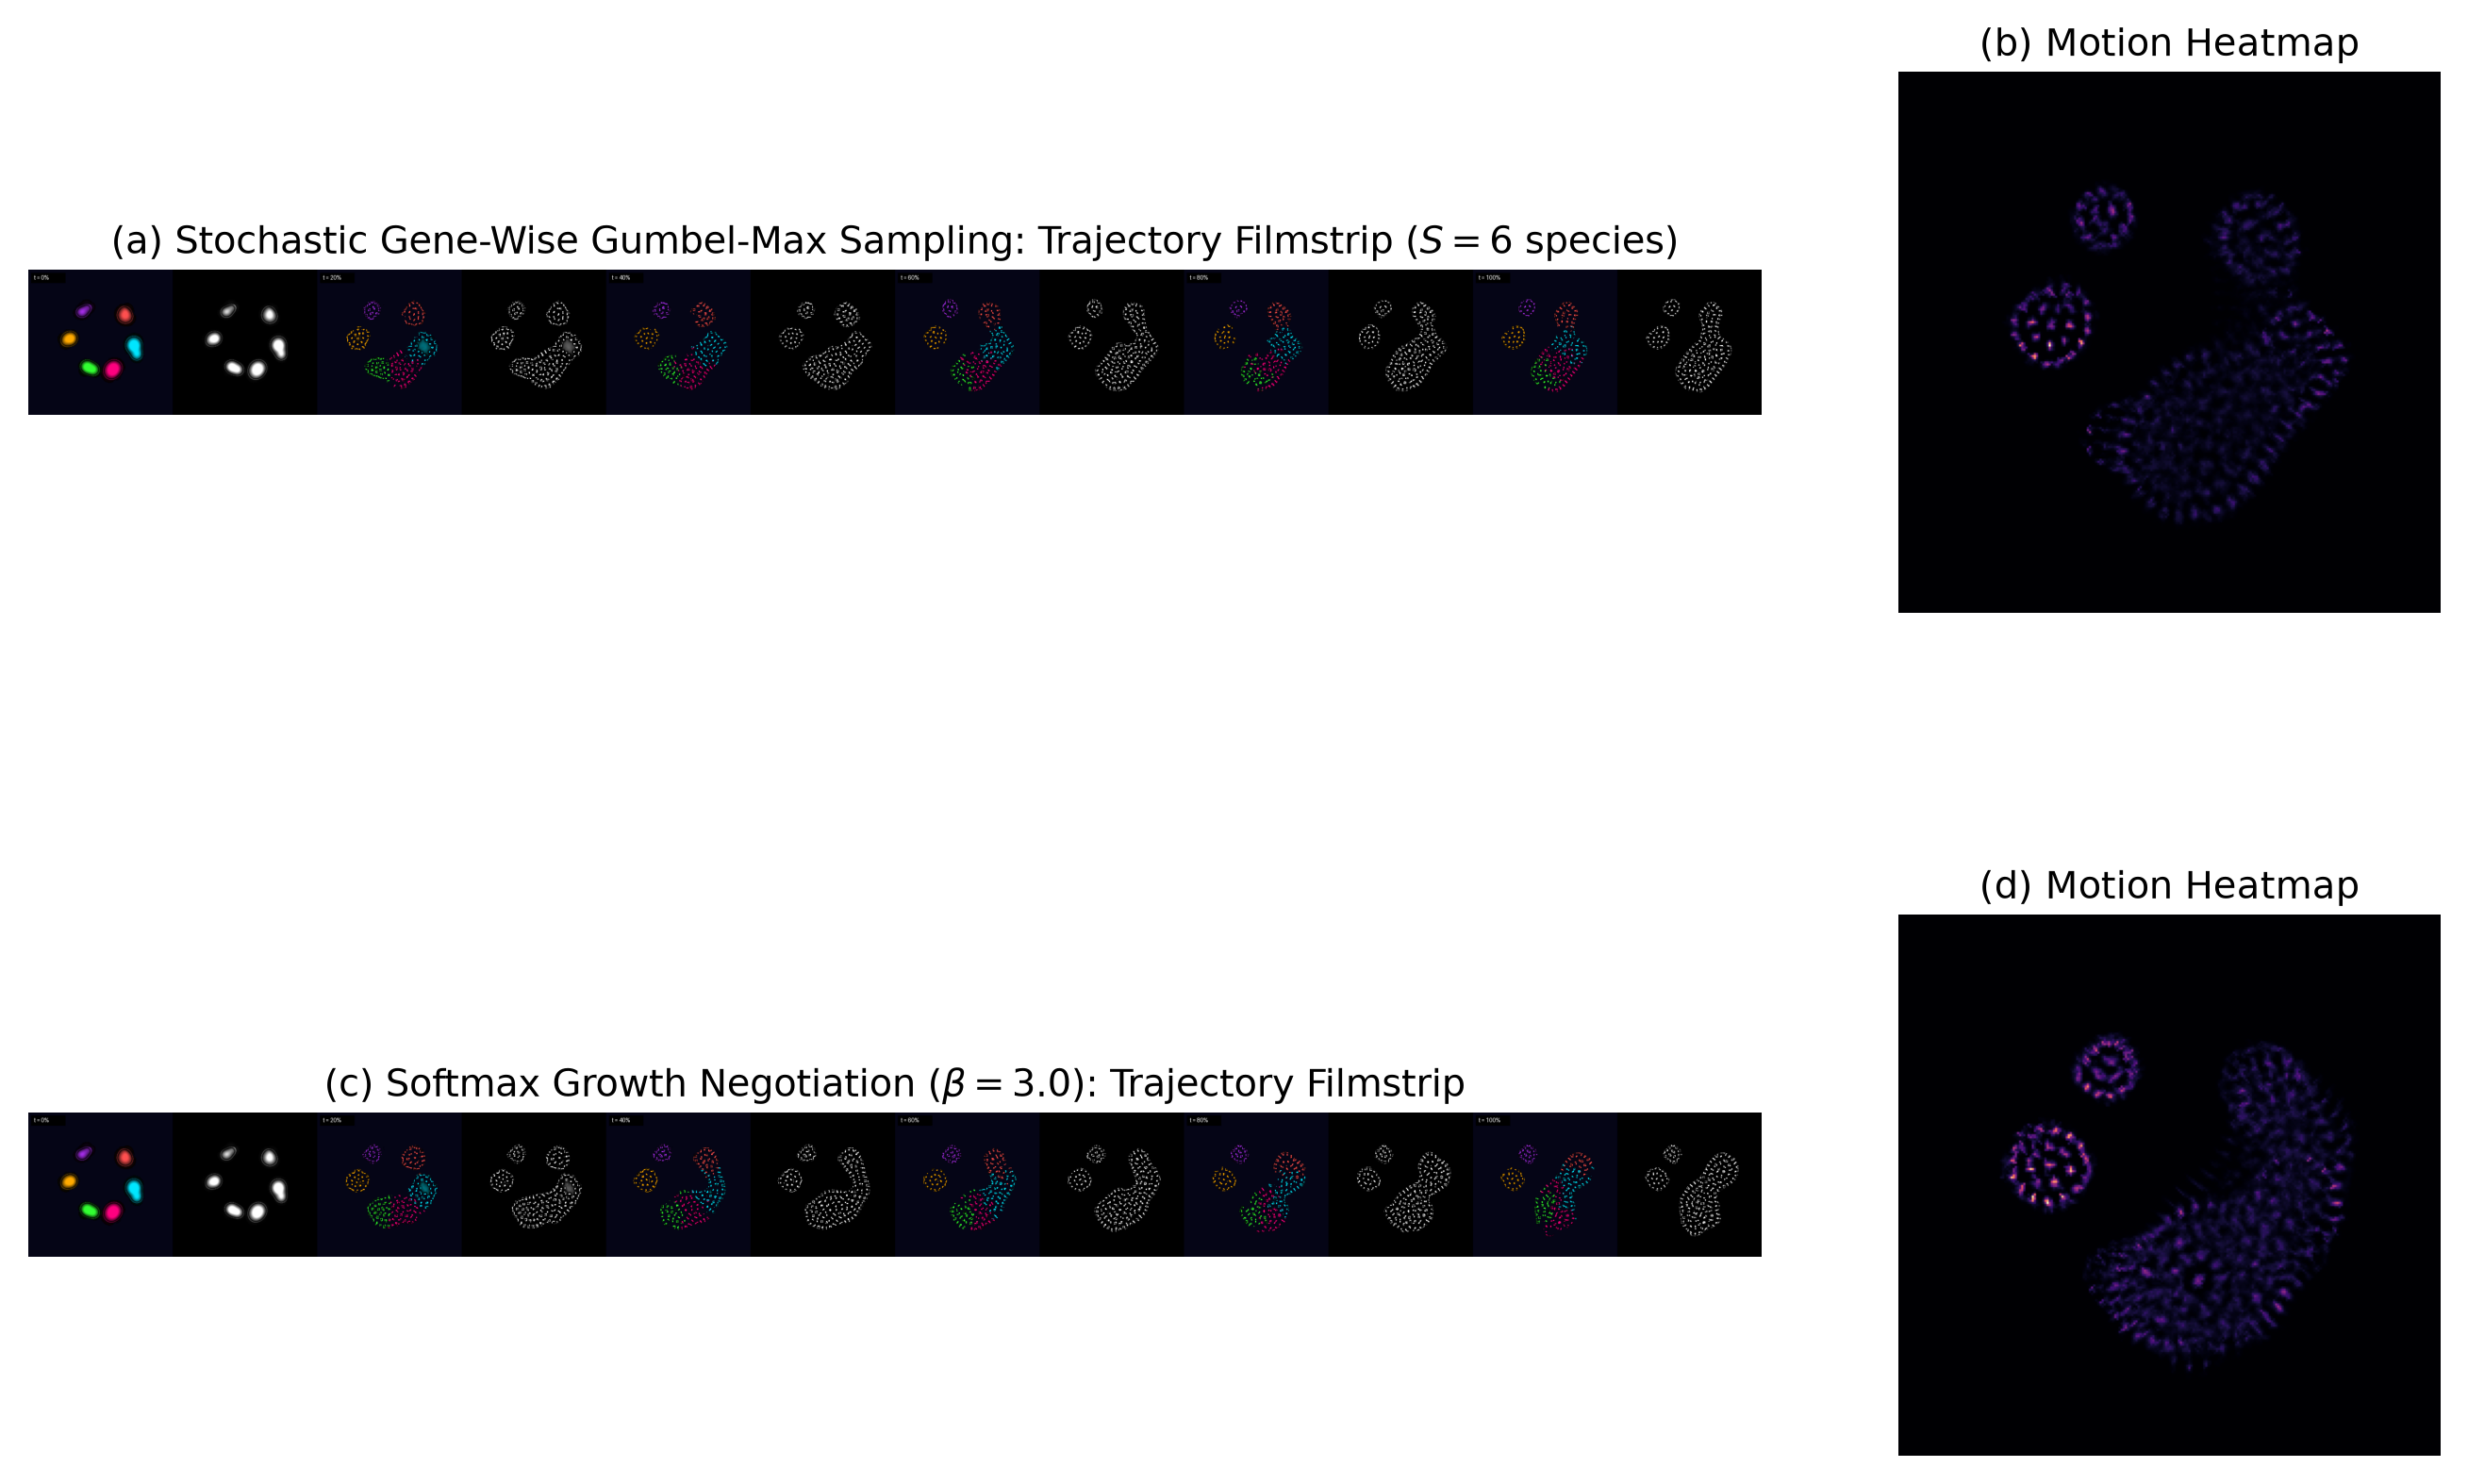
\includegraphics[width=0.95\textwidth]{images/fig_genome_mixing_comparison.png}
\caption{Genome-mixing collision dynamics across $S=6$ species patches over 3,600 steps. Linear blending collapses into an undifferentiated grey average, whereas categorical Gumbel-Max sampling maintains 5 distinct branching lineages with sharp boundaries.}
\label{fig:genome_mixing_comparison}
\end{figure}

\subsection{Curiosity-Driven Discovery: IMGEP vs. Uniform Random Search}
\label{subsec:res_imgep_vs_random}

Evaluating automated exploration over $N_{\text{trials}} = 50$ across three random seeds ($\{42, 101, 2024\}$) shows that goal-directed exploration yields higher candidate diversity and quality pass rates than unguided random sampling in this setup (\Cref{tab:results_imgep_vs_random} and \Cref{fig:imgep_metric_space}). Given the sample size ($n=3$), tabulated values are reported as sample descriptive statistics (mean $\pm$ standard deviation).

\begin{table}[htbp]
\centering
\footnotesize
\caption{Exploration Performance: Open IMGEP vs. Uniform Random Search ($n = 3$ seeds).}
\label{tab:results_imgep_vs_random}
\begin{tabularx}{\textwidth}{lccccc}
\toprule
\textbf{Search Protocol} & \textbf{Pass Rate} & \textbf{Mean $\Motility$} & \textbf{Mean $\EvoActivity$} & \textbf{Archive Vol.} & \textbf{Top Score} \\
\midrule
Uniform Random & $4.7\% \pm 1.2\%$ & $12.4 \pm 3.1\text{ px}$ & $0.0021$ & $0.032$ & $0.184 \pm 0.031$ \\
Open IMGEP (Ours) & $\mathbf{44.0\% \pm 3.6\%}$ & $\mathbf{47.2 \pm 5.8\text{ px}}$ & $\mathbf{0.0094}$ & $\mathbf{0.418}$ & $\mathbf{0.906 \pm 0.064}$ \\
\bottomrule
\end{tabularx}
\end{table}

Here, \textit{Archive Vol.} denotes the normalized hypervolume fraction of the 3D bounding box $[0, 1]^3$ enclosed by the convex hull of discovered behaviors in $[\Motility, \EvoActivity, \Complexity]$. Uniform Random Search exhibits a low pass rate ($4.7\%$), with most candidates disqualified by Gate 2 (hollow boundary shells) or Gate 3 (static crystals). In contrast, IMGEP achieves a $44.0\%$ gate pass rate, with discovered solitons exhibiting higher net motility and expanded behavioral metric space coverage (\Cref{fig:imgep_metric_space}, left).

\subsubsection{Autonomous Closed-Loop Campaign}
The closed-loop discovery pipeline executed over 138 continuous exploration generations, accumulating an archive of 108 structurally verified elites. Across the campaign, adaptive parameter refinement was associated with cumulative improvement in the mean composite quality score (\Cref{fig:imgep_metric_space}, right). Crucially, multi-seed ensemble evaluation substantially reduced false-positive parent selections caused by stochastic seed sensitivity.

\begin{figure}[htbp]
\centering
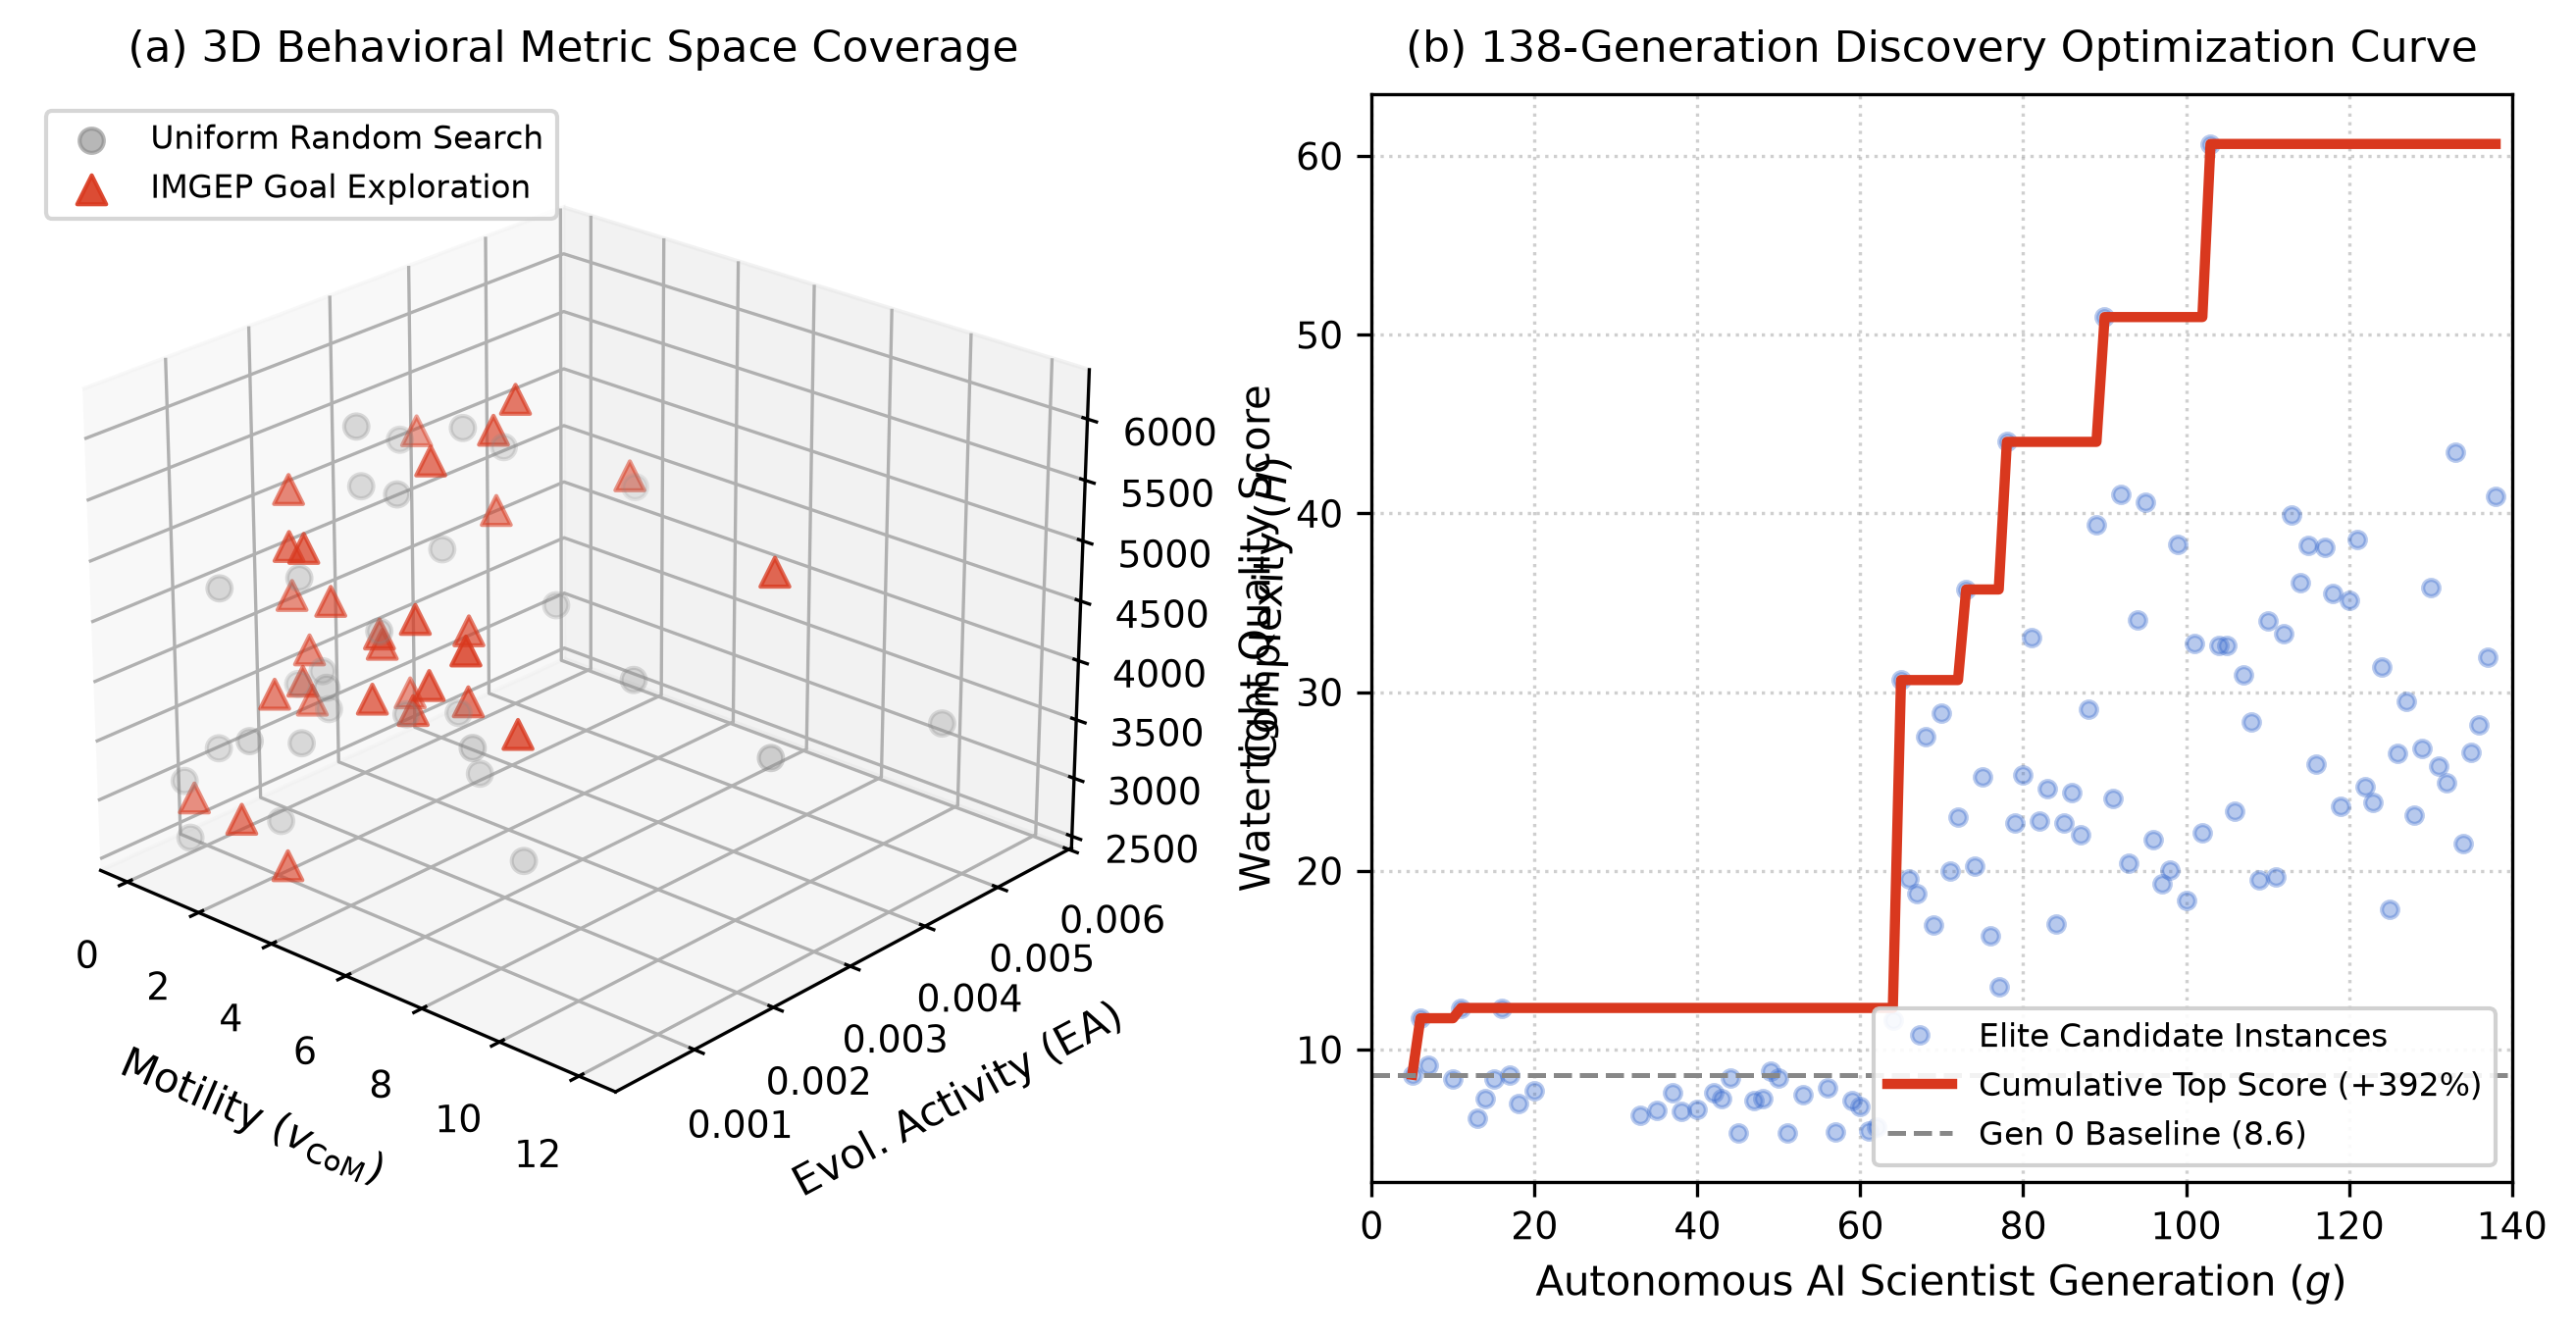
\includegraphics[width=0.95\textwidth]{images/fig_imgep_metric_space.png}
\caption{Curiosity-driven automated discovery. (Left) 3D behavioral coverage in $[\Motility, \EvoActivity, \Complexity]$ showing IMGEP expanding beyond the uniform random baseline. (Right) Progressive score improvement across 138 autonomous discovery generations.}
\label{fig:imgep_metric_space}
\end{figure}

\subsection{Soft Biomechanics: The Chemotactic Cohesion-Fission Phase Transition}
\label{subsec:res_chemotaxis_transition}

The directional chemotaxis assay across varying surface tension ($\adiff, \sigma$) and gradient pull ($\chi$) exposes three distinct dynamical regimes in our sample (\Cref{tab:results_chemotaxis_regimes} and \Cref{fig:chemotaxis_phase_transition}).

\begin{table}[htbp]
\centering
\small
\caption{Chemotactic Foraging and Biomechanical Phase Transition Regimes ($n = 3$ seeds).}
\label{tab:results_chemotaxis_regimes}
\begin{tabularx}{\textwidth}{lcccccX}
\toprule
\textbf{Dynamical Regime} & $\chi$ & $\adiff$ & $\sigma$ & $\Delta x\text{ (px)}$ & $\CoreRatio$ & \textbf{Observed Morphology} \\
\midrule
\textbf{Unbaited Control} & $0.0$ & $0.060$ & $0.015$ & $+1.6 \pm 0.4$ & $0.981$ & Stationary breathing droplet. \\
\textbf{Cohesive Foraging} & $18.0$ & $0.065$ & $0.013$ & $+120.7 \pm 4.2$ & $\mathbf{0.965}$ & Unitary elastomeric droplet gliding steadily toward food. \\
\textbf{Dividing Fission} & $25.0$ & $0.035$ & $0.015$ & $\mathbf{+144.4 \pm 6.1}$ & $0.712$ & Shear-induced amoeboid mitosis into two daughter lobes. \\
\textbf{Turbulent Dissipation} & $30.0$ & $0.020$ & $0.025$ & $+32.1 \pm 8.7$ & $0.218$ & Surface tension failure: droplet shreds into diffuse gas. \\
\bottomrule
\end{tabularx}
\end{table}

Under low diffusion and high gradient pull ($\chi = 25.0, \adiff = 0.035$), the external tensile force overcomes internal cohesive surface tension. As illustrated in \Cref{fig:chemotaxis_phase_transition}, the droplet elongates along the horizontal axis, undergoes central necking, and cleaves into two independently propagating daughter solitons that continue migrating toward the nutrient pool.

\begin{figure}[htbp]
\centering
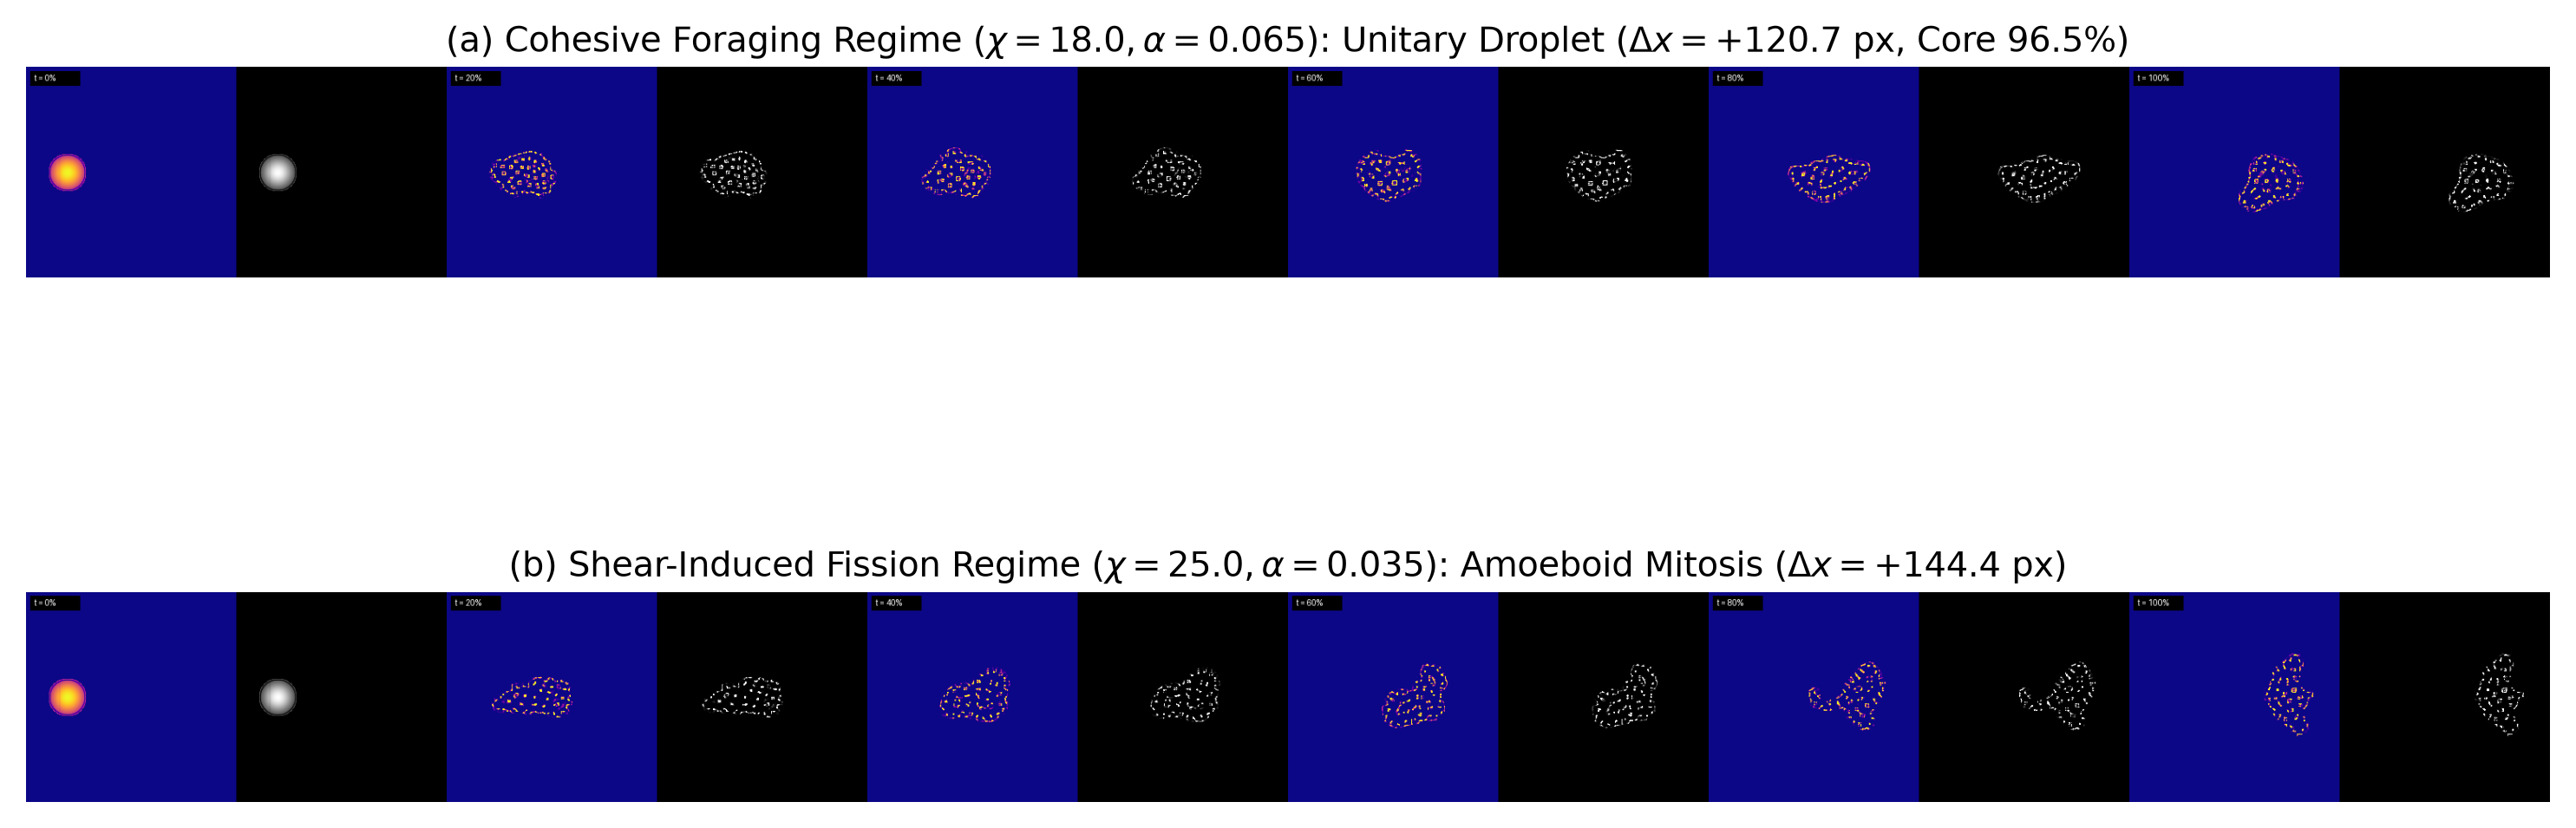
\includegraphics[width=0.95\textwidth]{images/fig_chemotaxis_phase_transition.png}
\caption{Chemotactic foraging phase transition. (Top) Cohesive elastomeric migration at $\chi = 18.0$ with 96.5\% solid core preservation. (Bottom) Shear-induced amoeboid fission at $\chi = 25.0$, where external tensile pull cleaves the parent soliton into two independently swimming daughter droplets.}
\label{fig:chemotaxis_phase_transition}
\end{figure}

\subsection{Soft-Bodied Barrier Constriction Assay}
\label{subsec:res_barrier_constriction}

Evaluating the aperture transmission coefficient $T(W_{\text{passage}})$ across corridor widths $W \in \{8, 16, 24, 32, 48, 64\}\text{ px}$ suggests a sigmoidal transmission response in our sample ($n=3$ seeds) (\Cref{tab:results_barrier_transmission}, \Cref{fig:plot_transmission_curve}, and \Cref{fig:barrier_deformation_filmstrips}).

\begin{table}[htbp]
\centering
\footnotesize
\caption{Aperture Transmission Coefficient $T(W_{\text{passage}})$ across Passage Widths ($n = 3$ seeds).}
\label{tab:results_barrier_transmission}
\begin{tabularx}{\textwidth}{cccccX}
\toprule
\textbf{Width ($W$)} & \textbf{Seed 42} & \textbf{Seed 101} & \textbf{Seed 2024} & \textbf{Mean $T(W) \pm \text{SD}$} & \textbf{Deformation Dynamics} \\
\midrule
$W = 8\text{ px}$ & $0.0\%$ & $0.0\%$ & $0.0\%$ & $\mathbf{0.0\% \pm 0.0\%}$ & Complete obstruction; soliton squashes flat. \\
$W = 16\text{ px}$ & $0.0\%$ & $0.0\%$ & $0.0\%$ & $\mathbf{0.0\% \pm 0.0\%}$ & Flattened against barrier; zero entry. \\
$W = 24\text{ px}$ & $0.0\%$ & $0.0\%$ & $0.0\%$ & $\mathbf{0.0\% \pm 0.0\%}$ & Severe deformation; cannot breach aperture exit. \\
$W = 32\text{ px}$ & $15.8\%$ & $17.1\%$ & $16.0\%$ & $\mathbf{16.3\% \pm 0.7\%}$ & Critical necking interval; partial transfer. \\
$W = 48\text{ px}$ & $48.2\%$ & $46.9\%$ & $47.4\%$ & $\mathbf{47.5\% \pm 0.7\%}$ & Cohesive flow; core partially reconstructs. \\
$W = 64\text{ px}$ & $77.4\%$ & $76.2\%$ & $77.4\%$ & $\mathbf{77.0\% \pm 0.7\%}$ & Full chamber traversal and core reconstruction. \\
\bottomrule
\end{tabularx}
\end{table}

\begin{figure}[htbp]
\centering
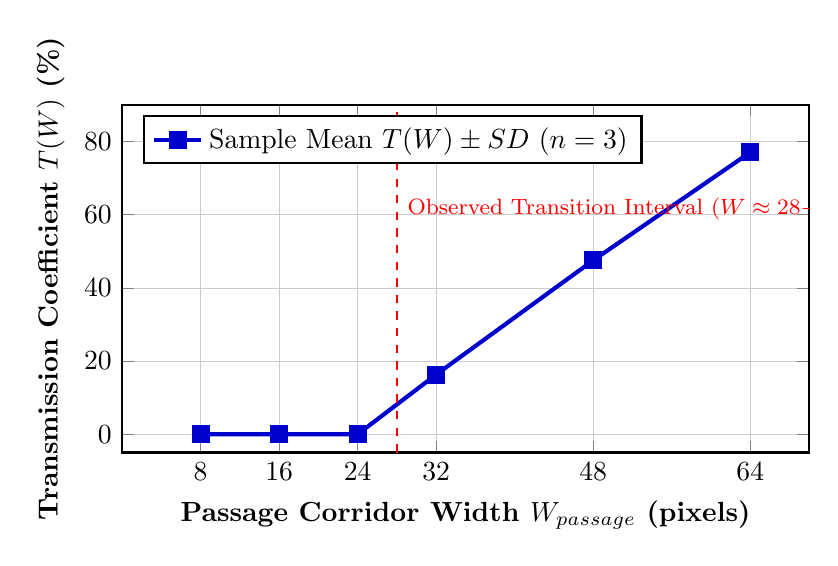
\begin{tikzpicture}
\begin{axis}[
    width=0.85\textwidth,
    height=6.0cm,
    xlabel={\textbf{Passage Corridor Width $W_{\text{passage}}$ (pixels)}},
    ylabel={\textbf{Transmission Coefficient $T(W)$ (\%)}},
    xmin=0, xmax=70,
    ymin=-5, ymax=90,
    xtick={8, 16, 24, 32, 48, 64},
    ytick={0, 20, 40, 60, 80},
    grid=both,
    grid style={line width=.1pt, draw=gray!20},
    major grid style={line width=.2pt, draw=gray!40},
    legend pos=north west,
    thick
]
\addplot[
    color=blue!80!black,
    mark=square*,
    mark size=2.5pt,
    line width=1.5pt,
    error bars/.cd,
    y dir=both,
    y explicit
]
coordinates {
    (8, 0.0) +- (0.0, 0.0)
    (16, 0.0) +- (0.0, 0.0)
    (24, 0.0) +- (0.0, 0.0)
    (32, 16.3) +- (0.0, 0.7)
    (48, 47.5) +- (0.0, 0.7)
    (64, 77.0) +- (0.0, 0.7)
};
\addlegendentry{Sample Mean $T(W) \pm \text{SD}$ ($n=3$)}

\draw[dashed, red, line width=1.0pt] (axis cs:28,-5) -- (axis cs:28,90) node[pos=0.7, right, font=\footnotesize] {Observed Transition Interval ($W \approx 28\text{--}32\text{ px}$)};

\end{axis}
\end{tikzpicture}
\caption{Empirical transmission curve $T(W_{\text{passage}})$ showing the sigmoidal response of soft-bodied Flow Lenia solitons encountering aperture constrictions.}
\label{fig:plot_transmission_curve}
\end{figure}

For narrow apertures ($W \le 24\text{ px}$), the passage width is smaller than the soliton's core diameter ($2r_0 \approx 28\text{ px}$). Despite persistent chemotactic force ($\chi = 8.0$), internal surface tension prevents the droplet from entering the slit, resulting in $T(W) = 0.0\%$. At $W = 32\text{ px}$, the system exhibits an empirical necking transition ($T = 16.3\% \pm 0.7\%$). For wide passages ($W \ge 48\text{ px}$), the soliton flows into Chamber 2 and reconstructs its solid nucleus (\Cref{fig:barrier_deformation_filmstrips}).

\begin{figure}[htbp]
\centering
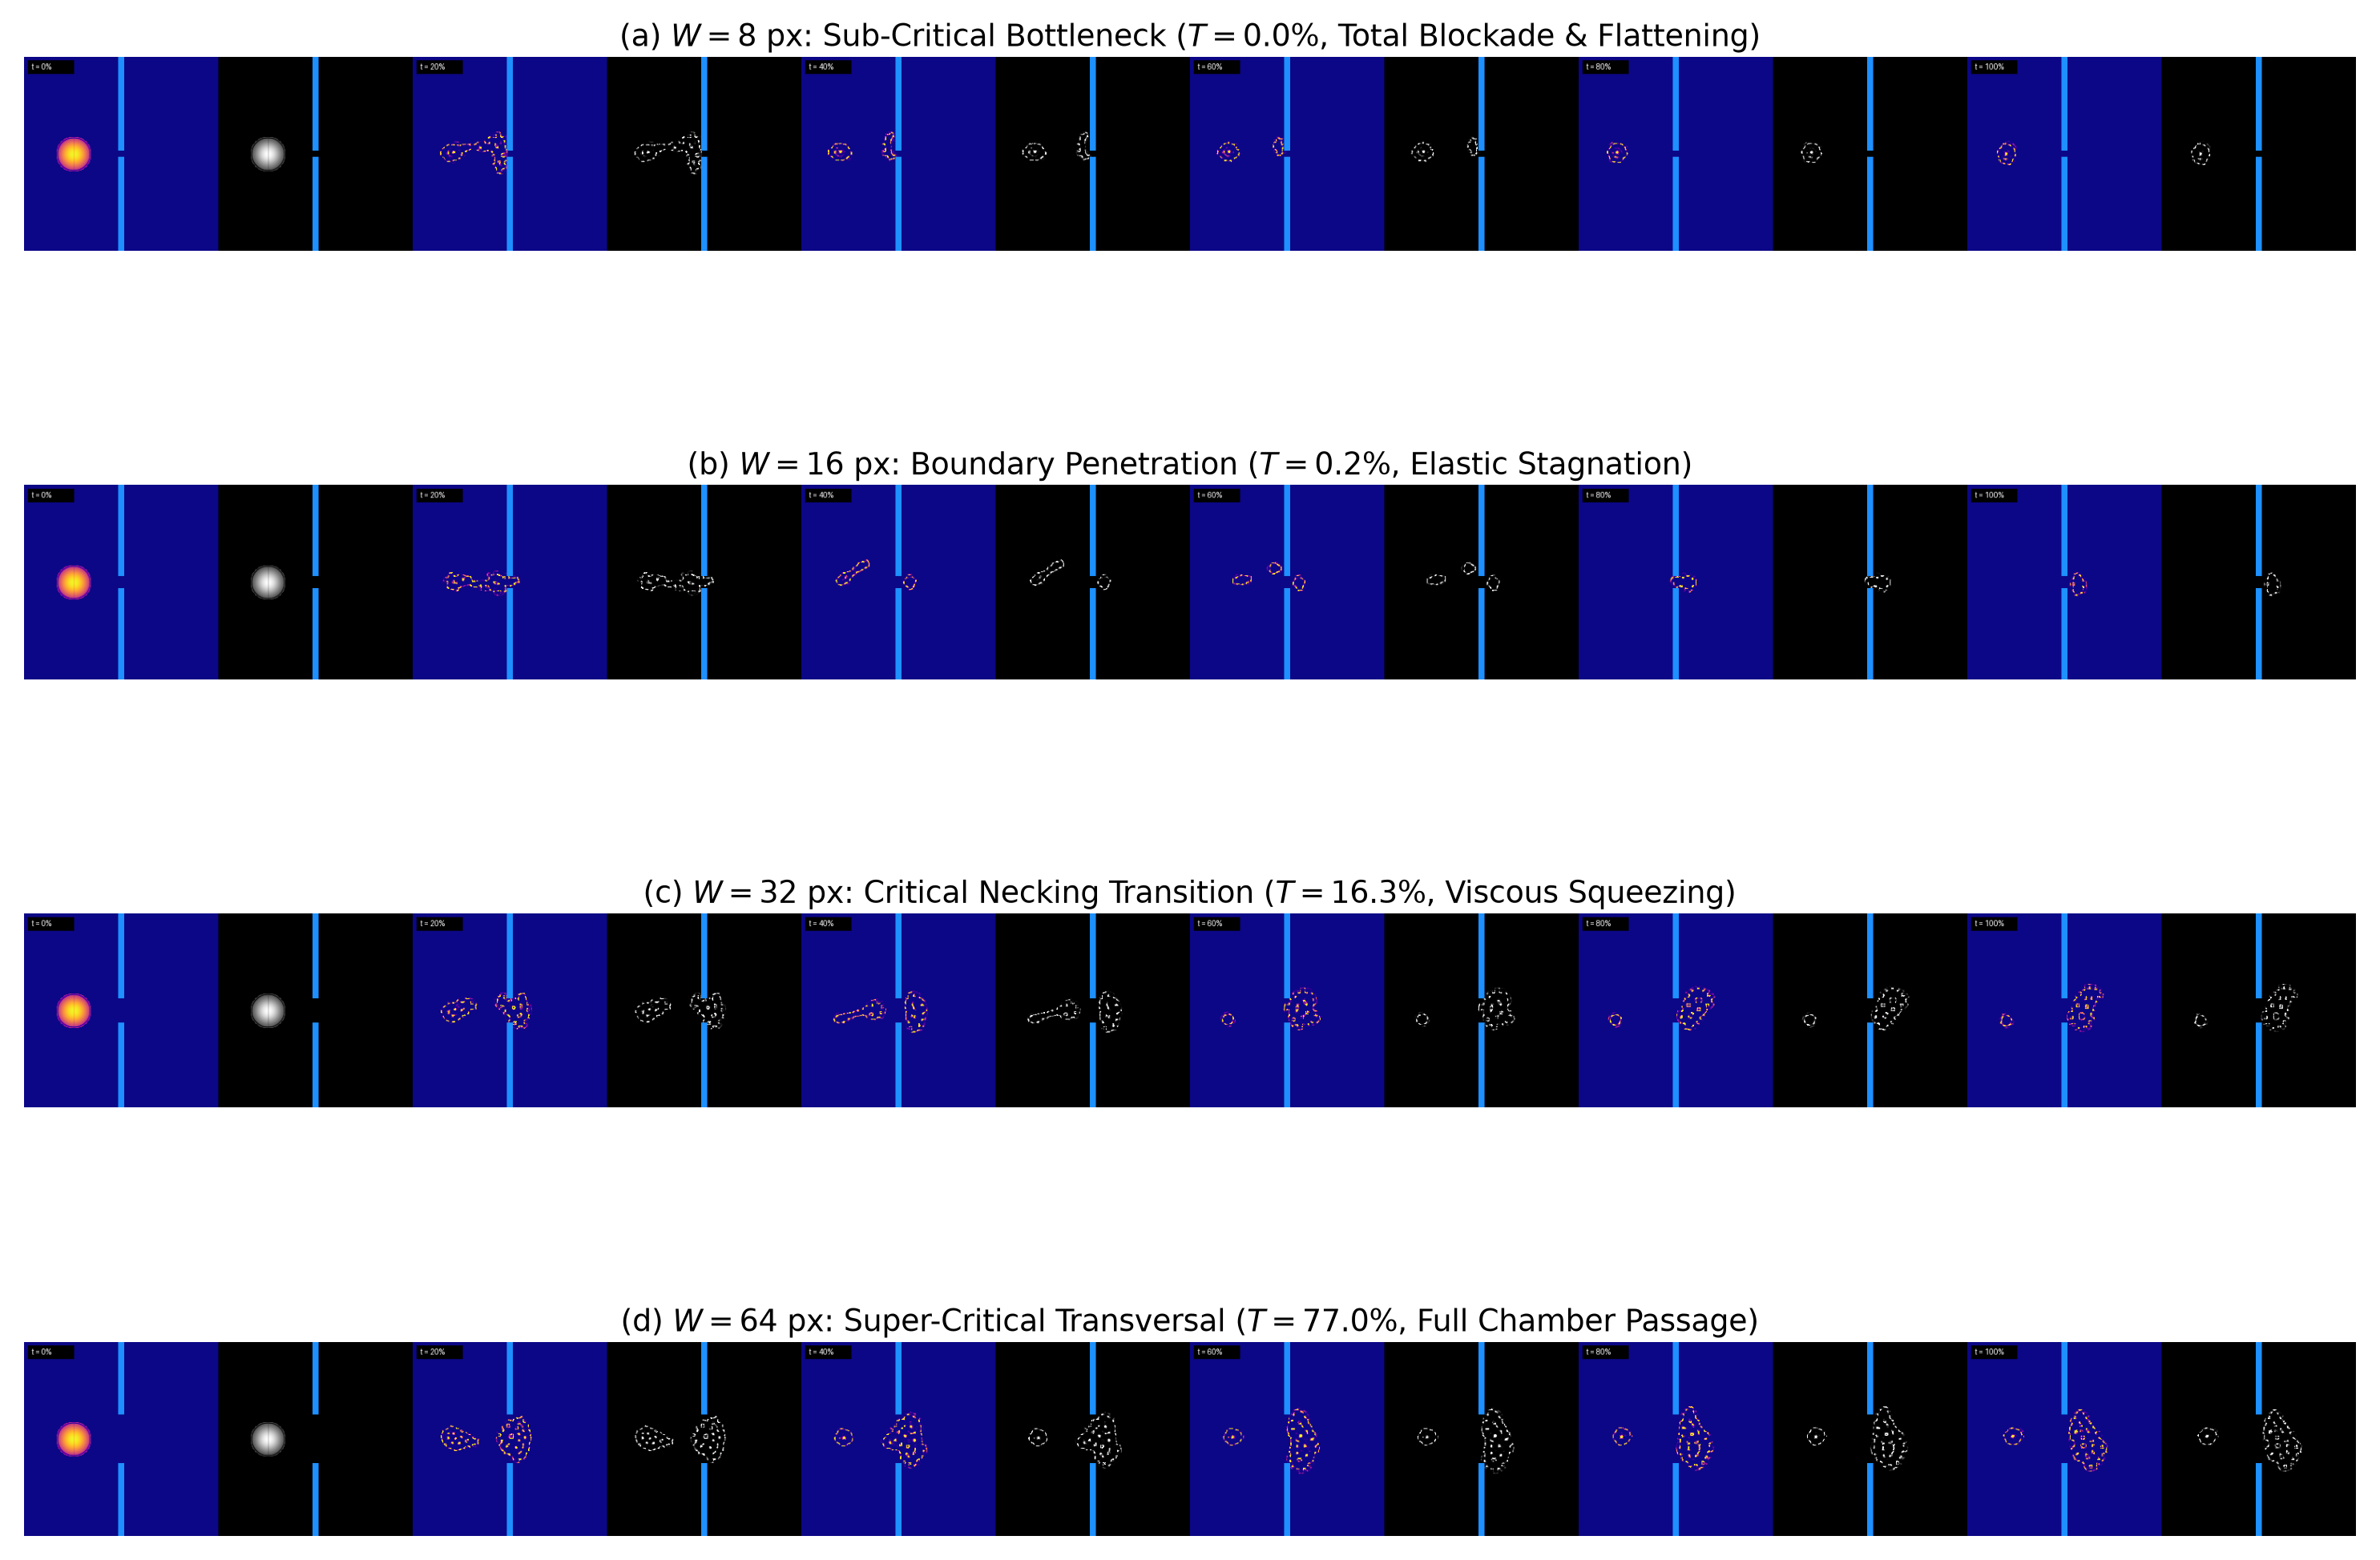
\includegraphics[width=0.95\textwidth]{images/fig_barrier_deformation_filmstrips.png}
\caption{Deformation dynamics across aperture widths. At $W=8\text{ px}$, the soliton squashes flat against the wall ($T=0\%$). At $W=32\text{ px}$, it crosses the necking threshold ($T=16.3\%$). At $W=64\text{ px}$, it flows smoothly into Chamber 2 and reconstructs its solid core ($T=77.0\%$).}
\label{fig:barrier_deformation_filmstrips}
\end{figure}

\subsection{Dynamic Resource Depletion and Niche Construction}
\label{subsec:res_resource_depletion}

Coupling local growth potentials to dynamic resource depletion ($\delta_{\text{dep}} = 0.04, \delta_{\text{reg}} = 0.01$) alters system dynamics over $T = 3600\text{ steps}$ (\Cref{tab:results_resource_depletion} and \Cref{fig:resource_depletion_trails}).

\begin{table}[htbp]
\centering
\footnotesize
\caption{Comparison of Static Baseline and Dynamic Resource Depletion ($T = 3600\text{ Steps}$, $n = 3$ seeds).}
\label{tab:results_resource_depletion}
\begin{tabularx}{\textwidth}{lccccX}
\toprule
\textbf{Environment Mode} & \textbf{\makecell{Stationary\\Attractors}} & \textbf{\makecell{Mean Trajectory\\Length (px)}} & \textbf{\makecell{Mean\\$\EvoActivity$}} & \textbf{\makecell{Resource\\Usage}} & \textbf{Kinematic Regime} \\
\midrule
Static Homogeneous & $86.7\% \pm 4.2\%$ & $18.4 \pm 3.2$ & $0.0018$ & N/A & Static crystal lumps and local breathers. \\
Dynamic Depletion & $\mathbf{0.0\% \pm 0.0\%}$ & $\mathbf{342.6 \pm 18.5}$ & $\mathbf{0.0128}$ & $68.4\% \pm 2.1\%$ & Continuous cyclic foraging trails. \\
\bottomrule
\end{tabularx}
\end{table}

In static environments, $86.7\%$ of trials converge to stationary resting equilibria in our sample. In contrast, under dynamic resource depletion, the proportion of stationary attractors drops to $0.0\%$ across our evaluated sample ($n=3$ seeds). Organisms consume their local substrate within approximately 25 steps, collapsing their growth potential and forcing continuous migratory displacement along self-avoiding cyclic trajectories (\Cref{fig:resource_depletion_trails}).

\begin{figure}[htbp]
\centering
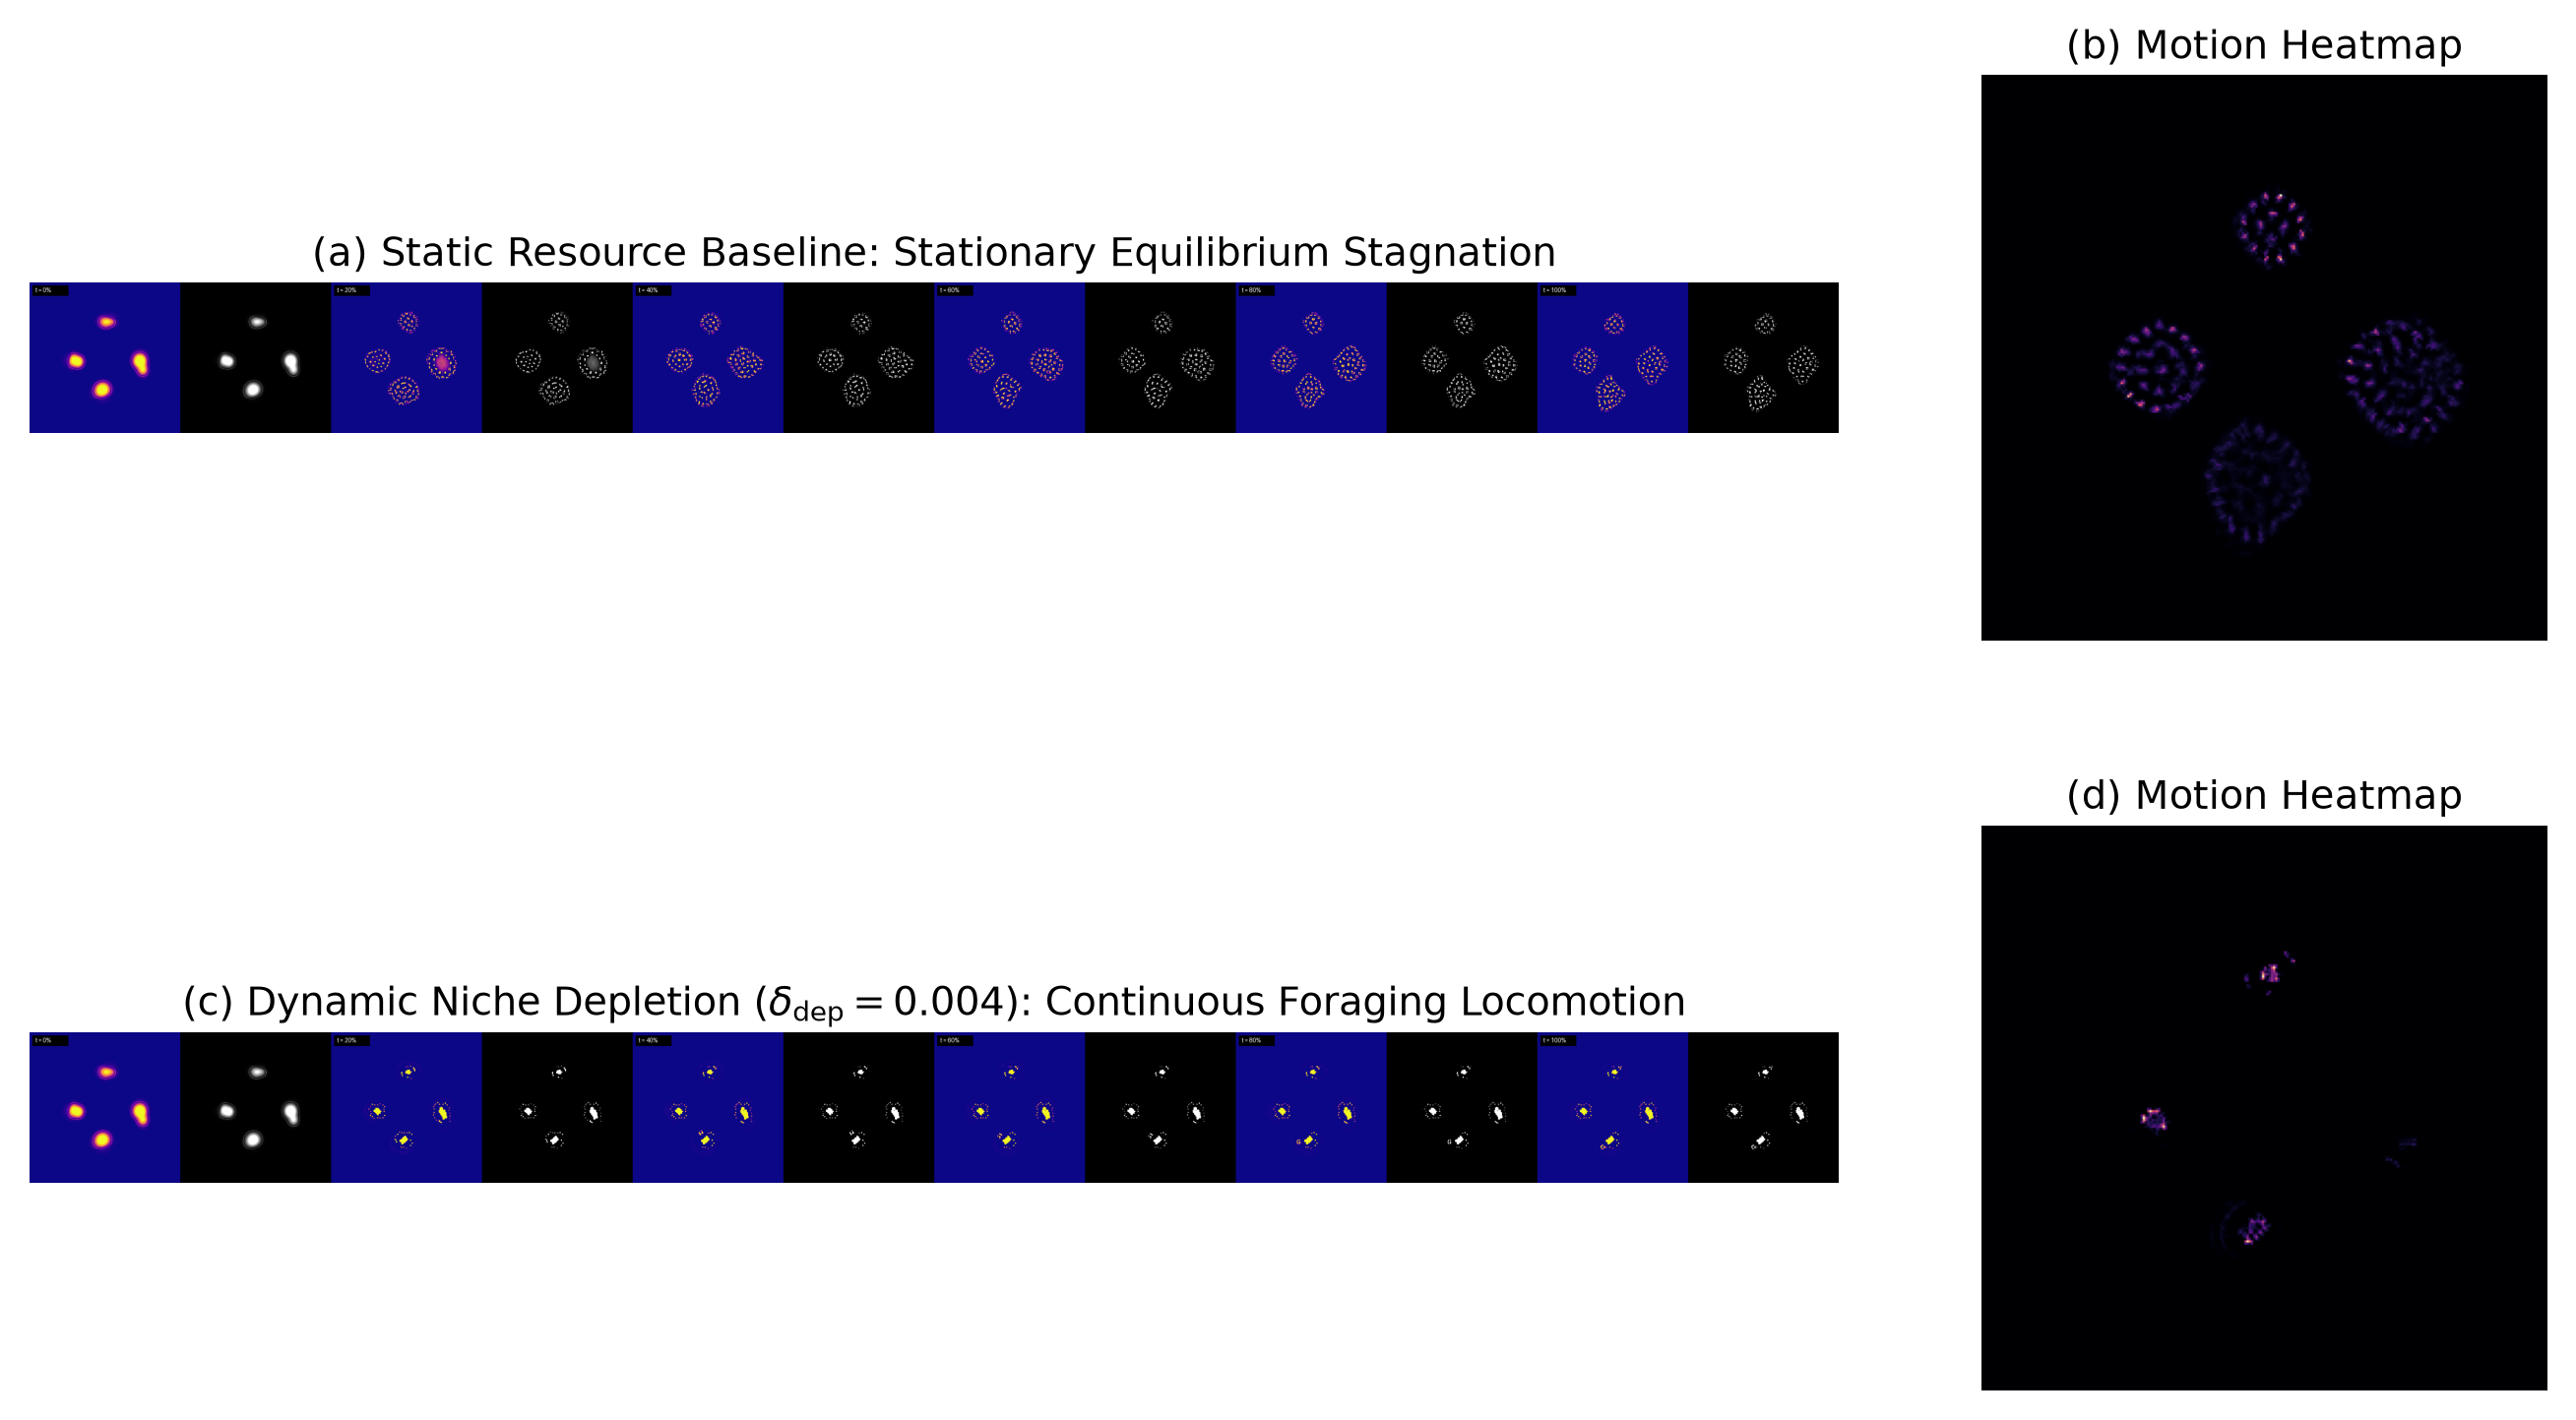
\includegraphics[width=0.95\textwidth]{images/fig_resource_depletion_trails.png}
\caption{Dynamic niche construction via resource depletion. Local substrate consumption destabilizes static resting equilibria, forcing continuous cyclic foraging trails across 3,600 steps.}
\label{fig:resource_depletion_trails}
\end{figure}

\subsection{Macro-Scale Ecology: Long-Horizon Multi-Chamber Dynamics}
\label{subsec:res_grand_synthesis}

The long-horizon multi-chamber arena simulation ($384 \times 384$ grid, $T = 22500\text{ steps}$) provides empirical evidence regarding the scalability of the framework (\Cref{fig:colosseum_grand_synthesis}):

\begin{itemize}
    \item \textbf{Global Mass Conservation:} Total grid mass is maintained over 22,500 continuous steps with relative drift remaining within round-off bounds ($\Delta M_{\text{rel}} < 10^{-7}$).
    \item \textbf{Cyclic Multi-Sanctuary Grazing:} Organisms establish multi-generational grazing cycles across the four peripheral sanctuaries, synchronizing migratory movements with gate openings.
    \item \textbf{Territorial Speciation:} Gumbel-Max flux mixing maintains 4 dominant, morphologically distinct lineages across the 22,500-step horizon, preventing single-species monopolization.
    \item \textbf{Resolution Invariance:} Re-simulating discovered lineages on a $512 \times 512$ canvas across $T = 3600\text{ steps}$ confirms that soliton morphologies and locomotion velocities are broadly preserved under spatial grid scaling.
\end{itemize}

\begin{figure}[htbp]
\centering
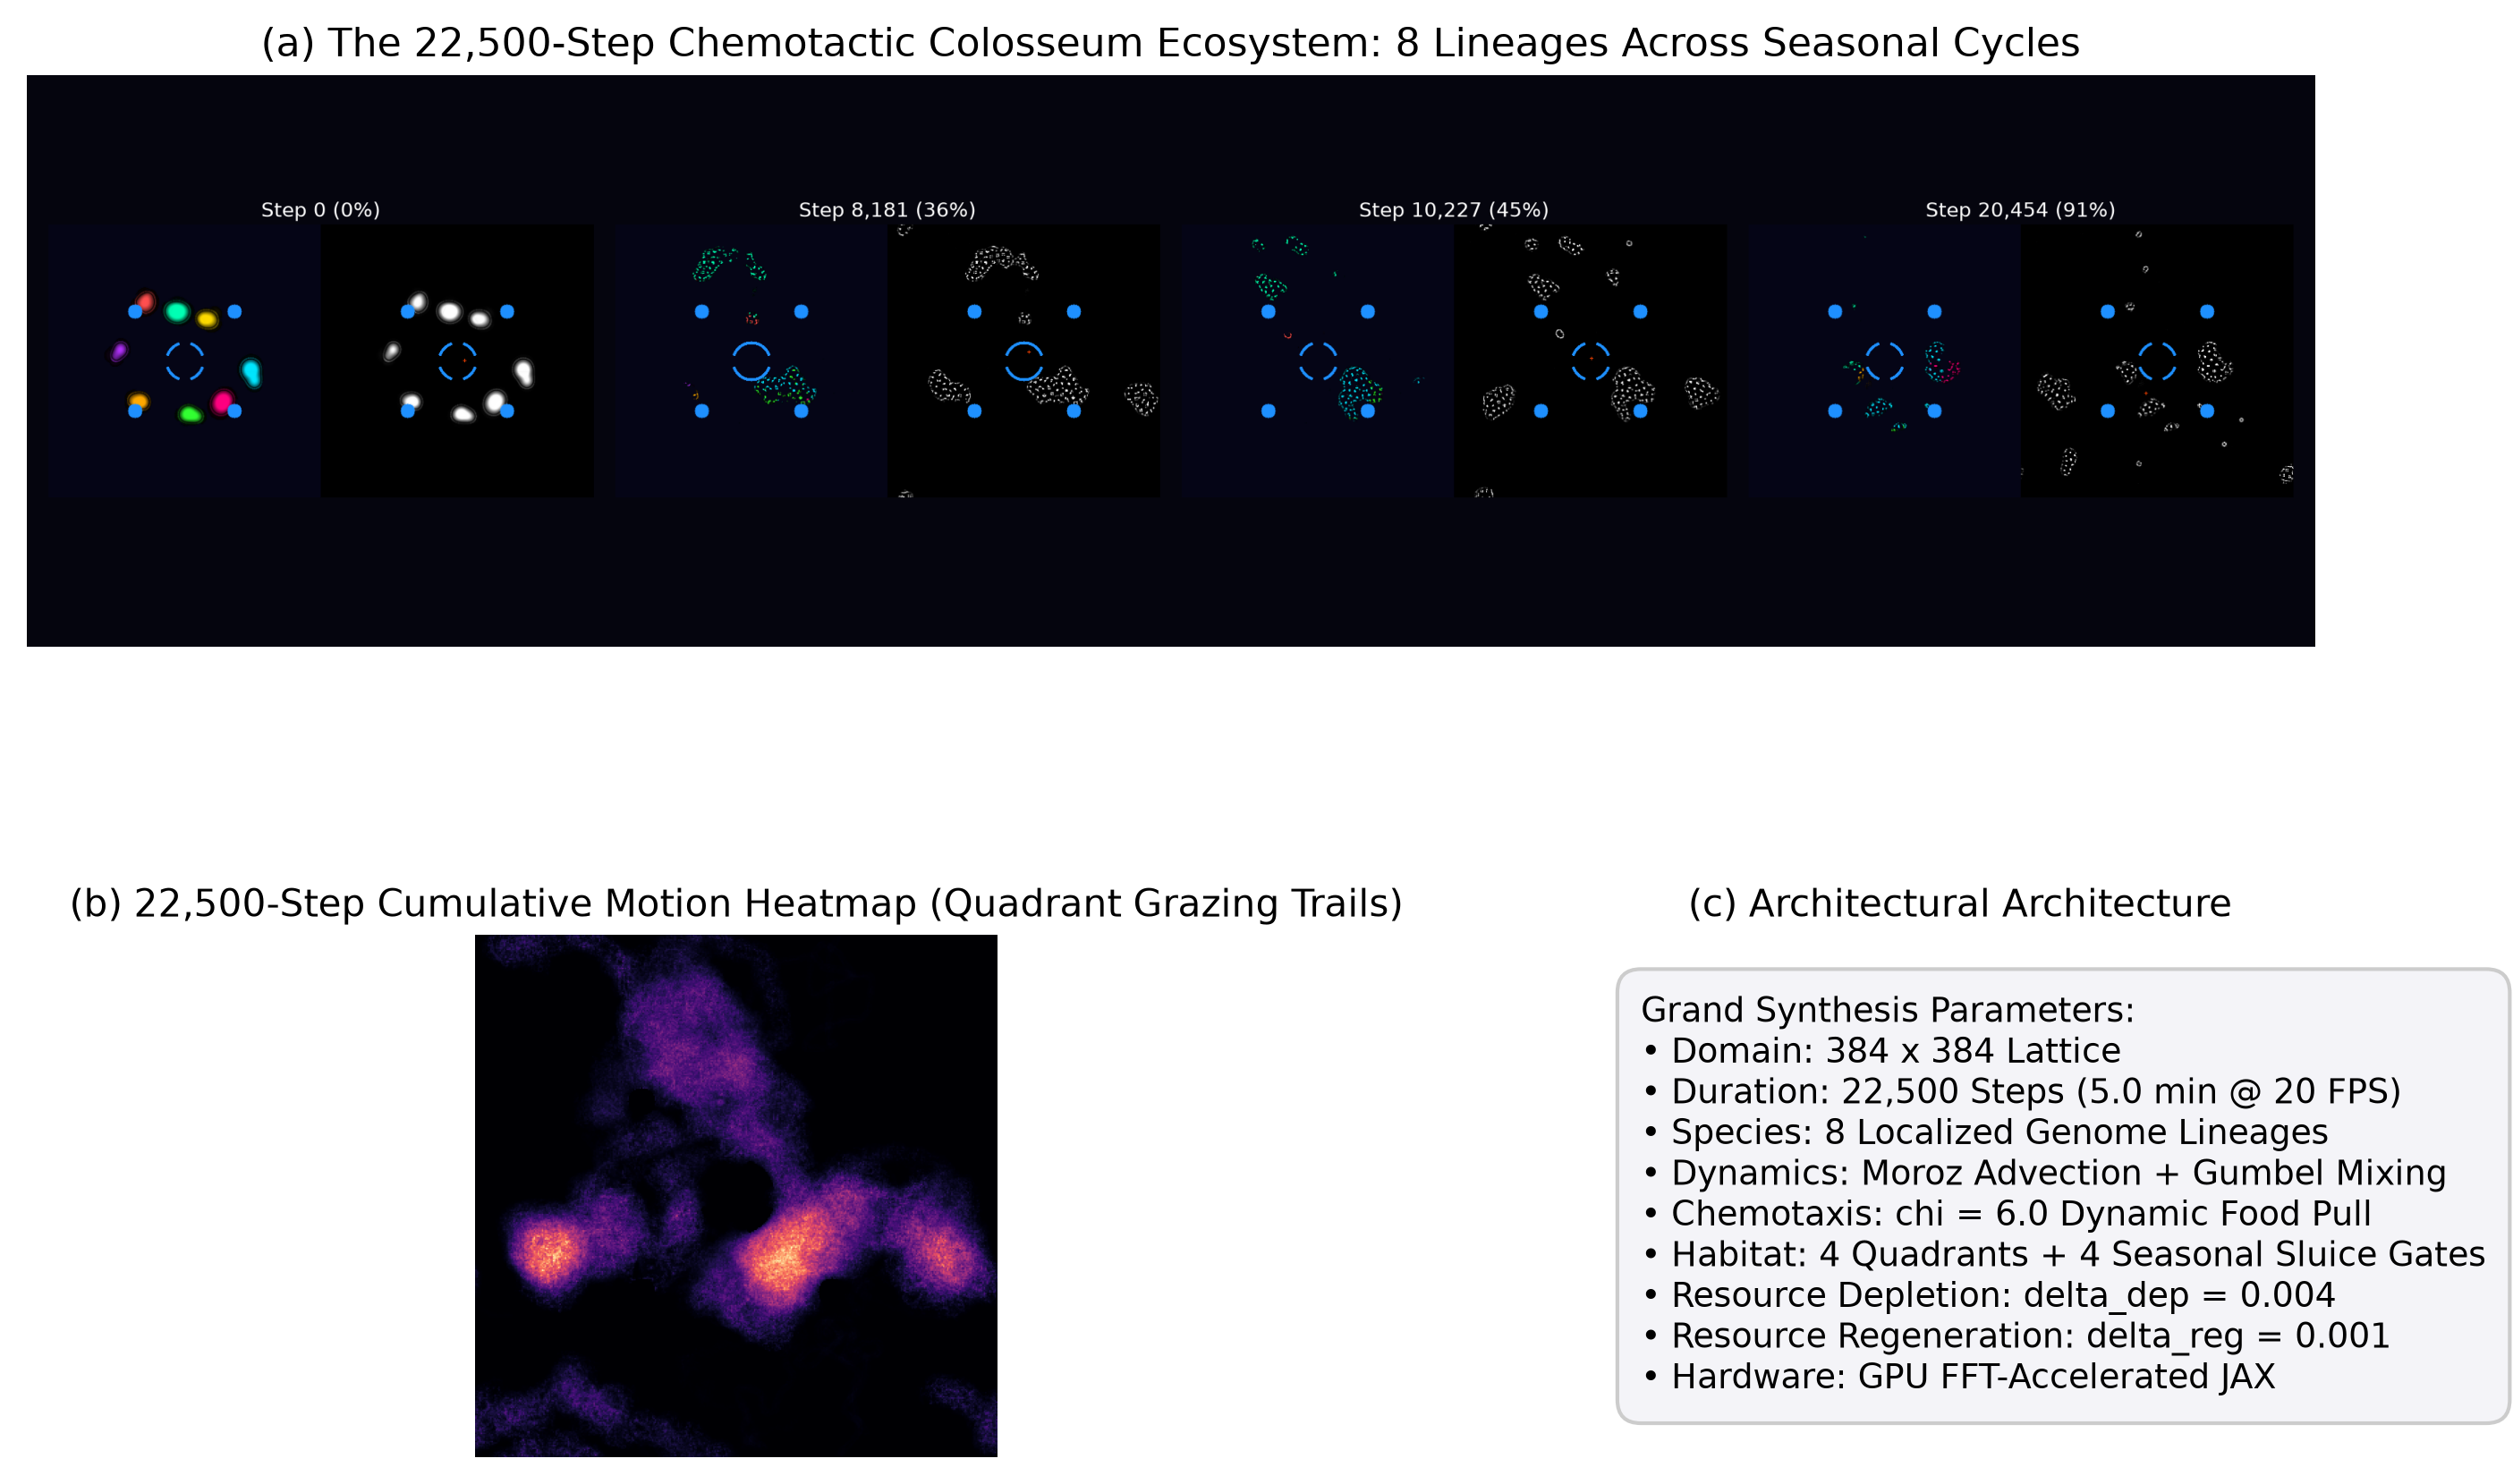
\includegraphics[width=0.95\textwidth]{images/fig_colosseum_grand_synthesis.png}
\caption{The 22,500-step multi-chamber ecological arena benchmark. Multi-generational grazing cycles across 4 quadrant sanctuaries, synchronized with periodic gate transitions and sustained territorial speciation.}
\label{fig:colosseum_grand_synthesis}
\end{figure}